\documentclass{article}
\usepackage{amssymb}
\usepackage[utf8]{inputenc}
\usepackage{amsmath}
\usepackage[spanish]{babel}
\usepackage{tikz}
\usepackage{graphicx}
\newcommand{\N}{\mathbb{N}}
\newcommand{\R}[1]{$\mathbb{R}^#1$}
\newcommand{\Phisub}[1]{$\varphi_#1$}
\newcommand{\matriz}[4]{\begin{pmatrix}
#1 & #2\\
#3 & #4
\end{pmatrix}}
\newcommand{\cauchy}[0]{
    \[(P) = \biggl\{ 
            \begin{array}{c}
            y' = f(t,y(t)) \\
            y(t_0) = y_0
            \end{array}
    \]
}
\newcommand{\defcauchy}{f: D \subseteq \mathbb{R}\times \mathbb{R}^n \rightarrow\mathbb{R}^n, \ t_0\in \mathbb{R}, \ y_0\in \mathbb{R}}
\newcommand{\phit}{\phi(t) = y_0 + \int_{t_0}^{t}f(s, \phi(s))\cdot ds}


\providecommand{\norm}[1]{\lVert#1\rVert}
\usepackage{amsthm}
\usepackage{graphicx}

\newtheorem{definition}{Definición}[section]
\newtheorem{observation}{Observación}[section]
\newtheorem{theorem}{Teorema}[section]
\newtheorem{proposition}{Proposición}[section]
\newtheorem{lemma}{Lema}[section]
\newtheorem{corollary}{Corolario}[section]
\newtheorem{example}{Ejemplo}[section]
\newtheorem{exercise}{Ejercicio}[section]



\title{	

	\normalfont\normalsize
	\textsc{Universidad de Murcia}\\ 
	\vspace{25pt} % Whitespace
	\rule{\linewidth}{0.5pt} % Thin top horizontal rule
	\vspace{20pt}\\ % Dará error hasta que escribas algo en el título
	{\huge EDO
}\\ % The assignment title
	\vspace{12pt} % Whitespace
	\rule{\linewidth}{2pt}\\ % Thick bottom horizontal rule
	\vspace{12pt} % Whitespace
	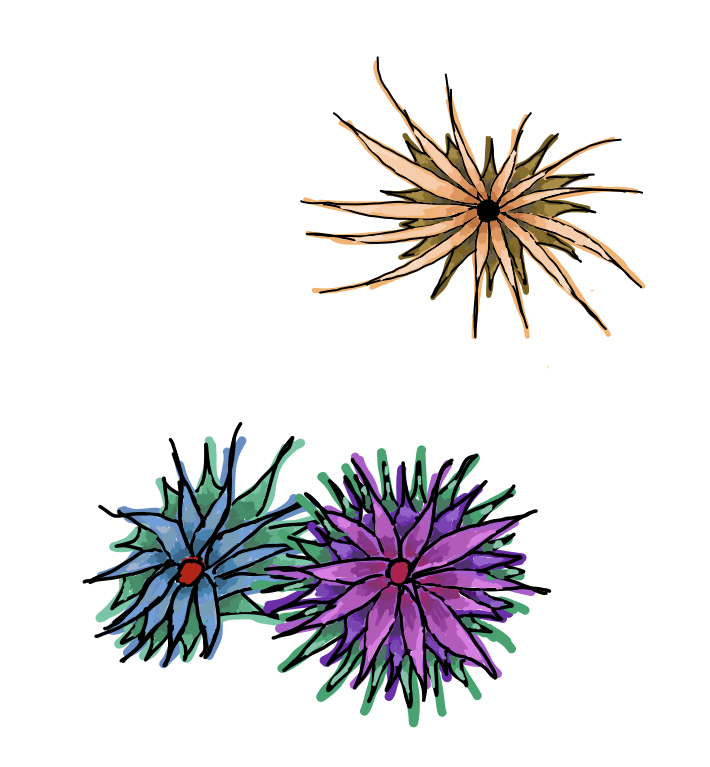
\includegraphics[scale=0.25]{floresportada.png}
}


\author{\LARGE Teresa \\ \LARGE Alonso Oma Alonso} % Your name

  
 
\date{\normalsize\today} % Today's date (\today) or a custom date



\begin{document}

\begin{titlepage}
	\maketitle
\end{titlepage}

\newpage
\tableofcontents
\newpage

\begin{section}{Tema 1: Introducción. Existencia y unicidad de soluciones.}

	\begin{subsection}{Introducción y definiciones}
        Las ecuaciones diferenciales son muy importantes por su aplicación en las ciencias experimentales y
        en las técnicas, y también, por supuesto, son muy importantes en Matemáticas. Son muchas las leyes de
        la naturaleza que se explican mediante las ecuaciones diferenciales, ya que estas expresan una relación
        entre una función y sus derivadas. No debemos olvidar que la derivada de una función expresa la variación
        de esta respecto de la variable de la que depende. En primer lugar veremos un ejemplo:
        $\bigskip$

        \textbf{\underline{Caída retarada de un objeto:}}
        Supongamos que tenemos un objeto de masa \textbf{m} que cae libremente por la acción de la gravedad y que
        el aire ejerce una fuerza de resistencia proporcional a la velocidad . La 2ª Ley de Newton dice \textit{"La
        fuerza resultante que actúa sobre un cuerpo es directamente proporcional a la masa y a la aceleración con que
        se mueve"} es decir, $\mathbf{\sum F = m \cdot a}$
        \[\overbrace{m \cdot a}^{F_1} = \overbrace{mg - k\cdot v}^{F_2}\]

        Supongamos que el cuerpo se encuentra a una cierta altura "\textbf{h}". Si denotamos por $y(t)$ a la función
        que nos da la posición del objeto en el instante "\textbf{t}" obtenemos la ecuación:
        \[m\cdot y''(t) = mg -k\cdot y'(t) \mathit{\quad Ecuaci\acute{o}n\ diferencial\ de\ segundo\ orden.}\]

        Si nos preguntamos cuál es la posición del objeto después de por ejemplo, 2 segundos, tendriamos que "resolver" la
        ecuación diferencial.
        $\bigskip$

        \textbf{\underline{Movimiento pendular:}}
        Supongamos que tenemos una varita de masa despreciable de longitud "\textbf{l}" y con un objeto de masa "\textbf{m}"
        en el extremo. Si impulsamos el péndulo hasta un ángulo "$\theta_0$" se tendrá que en la posición extrema $\theta = \theta_0$
        sólo tiene energía potencial:
        \[E = mg(l-l\cos \theta_0)\]

        En la posición $\theta(t)$ la energía del péndulo es parte cinética y parte potencial:
        \[E = \frac{1}{2}mv^2 + mg(l-l\cos\theta(t))\]

        El \textit{\textbf{"Principio de conservación de la energía"}} dice que la energía se conserva y por lo tanto:
        \[\frac{1}{2}mv^2\ = mg(l\cos\theta(t)-l\cos\theta_0)\]

        Si denotamos por $s(t)$ a la longitud del arco correspondiente al ángulo $\theta(t)$ entonces $s(t) = l\cdot \theta(t)$ y $v(t) = l\cdot \theta'(t)$.

        Sustituyendo en la ecuación anterior tenemos :
        \[\frac{1}{2}ml^2(\theta'(t))^2 = mgl(\cos\theta(t)-\cos\theta_0) \Rightarrow (\theta'(t))^2=\frac{2g}{l}(\cos\theta(t)-\cos \theta_0)\]

        es decir,
        \[\theta'(t)\ = -\ \sqrt[]{\frac{2g}{l}(\cos\theta(t)-\cos \theta_0)}\mathit{\quad Ecuaci\acute{o}n\ diferencial\ de\ primer\ orden.} \]
		
        \textit{Nota: Se toma el valor negativo pues $\theta(t)$ disminuye en función del tiempo.}
        $\bigskip$

        \begin{definition}
            {Ecuación diferencial:}
            Una ecuación diferenciales una ecuación en la que la incógnita es una función/funciones
            y en la que aparacen las derivadas ó derivadas parciales de la función/funciones
            con respecto a su variable /variables independientes.
    
            \begin{itemize}
                \item \textbf{Ecuación diferencial ordinaria} $\longrightarrow$ e.d. con una sola variable independiente.
                \item \textbf{Ecuaciones en Derivadas Parciales} $\longrightarrow$ e.d. con dos o más variables independientes.
            \end{itemize}
        \end{definition}
    
        En este curso estudiaremos las ecuaciones diferenciales ordinarias.
    
        \begin{definition}
            {EDO escalar}
    
            Una ecuación diferencial ordinaria 'escalar' de orden n es una expresión de la forma:
    
            \[F(t, y(t), y'(t), \dots, y^{(n)}(t)) = 0\]
    
            donde 
            \begin{itemize}
                \item $F: \Omega \subseteq \mathbb{R} \times \mathbb{R}^{n+1} \longrightarrow \mathbb{R}$, 
                \item $t$ es la variable independiente,
                \item $y(t), y'(t), \dots, y^{(n)}$ es la variable dependiente o \textbf{función desconocida}
                $y: I \rightarrow \mathbb{R}$ y sus derivadas sucesivas respectode t.
            \end{itemize}
    
            La forma anterior se llama \textbf{forma explícita} de la EDO de orden n.
    
            La forma \textbf{normal o explícita} de una EDO de orden n es cuando se encuentra resuelta
            con respecto de la derivada de orden n de la función, es decir,
    
            \[y^{(n)}(t) 0 f(t, y(t), y'(t), \dots, y^{(n-1)}(t))\]
    
            donde $f: D \subset \mathbb{R} \times \mathbb{R}^n \longrightarrow \mathbb{R}$.
    
            \textbf{Nota: } El orden de una ED es el de su derivada de mayor orden.
    
        \end{definition}
    
        Ahora se plantean las cuestiones: ¿cómo se resuelve una ED. Ordinaria? ¿Qué
        se considera una solución?
    
        \begin{definition}
    
            Sea \textcolor{red}{$\bigotimes$} $F(t, y, y', \dots, y^{n}) = 0$ una EDO de orden n.
        
            \[F: \Omega \subseteq \mathbb{R} \times \mathbb{R}^{n+1} \longrightarrow \mathbb{R}\]
    
            Se dice que $\phi : I \rightarrow \mathbb{R}$ es solución de \textcolor{red}{$\bigotimes$} en $I$ ($I$ intervalo de $\mathbb{R}$)
            si cumple:
    
            \begin{itemize}
                \item $\phi$ es derivable n veces en $I$.
                \item $(t, \phi (t), \phi'(t), \dots, \phi^{(n)}(t)) \in \Omega, \quad \forall t \in I$.
                \item $F(t, \phi(t), \phi'(t), \dots, \phi^{(n)}) = 0, \quad \forall t \in I$.
            \end{itemize}
    
    
            Hay EDOs que no tienen solución, las hay que tienen infinitas soluciones  y las hay que sólo tienen una.
        \end{definition}
    
        Lo más usual es que la EDO tenga $\infty$ soluciones que dependen de parámetros.
    
        \begin{subsection}{\textbf{EDO's escalares y EDO's vectoriales}}
            \begin{definition}{EDO escalar ($y: I \subseteq \mathbb{R} \rightarrow \mathbb{R}$):}
                
                \[\begin{array}{ccc}
                    F(t, y(t), y'(t), \dots, y^{(n)}(t)) = 0& \quad & y^{(n)}(t) = f(t, y(t), y'(t), \dots, y^{(n-1)}(t)) \\
                    F:\Omega \subseteq \mathbb{R} \times \mathbb{R}^n \rightarrow \mathbb{R}& \quad & f:D \subseteq \mathbb{R}^n \rightarrow \mathbb{R}
                \end{array}\]
            \end{definition}
    
            \begin{definition}
                EDO vectorial ($y: I \subseteq \mathbb{R} \rightarrow \mathbb{R}^m$):
    
                \[\begin{array}{ccc}
                    F(t, y(t), y'(t), \dots, y^{(n)}(t)) = 0& \  & y^{(n)}(t) = f(t, y(t), y'(t), \dots, y^{(n-1)}(t)) \\
                    F:\Omega \subseteq \mathbb{R} \times \overbrace{\mathbb{R}^m \times \dots \times \mathbb{R}^m}^{(n+1)-\text{veces}} \rightarrow \mathbb{R}& \ & f:D \subseteq \mathbb{R} \times \overbrace{\mathbb{R}^m \times \dots \times \mathbb{R}^m}^{(n)-\text{veces}} \rightarrow \mathbb{R}
                \end{array}\]
            \end{definition}
        \end{subsection}
    
        \begin{definition}{\textbf{Sistemas de ecuaciones diferenciales ($Y: I\subseteq \mathbb{R} \rightarrow \mathbb{R}^m$)}}
            
            Considerando las funciones componentes, toda función vectorial se transforma en un sistema de ecuaciones diferenciles y al revés.
            $\bigskip$
    
            \textbf{\textcolor{red}{Importante:} Toda EDO escalar de orden 'n' se puede transformar mediante un 'cambio de variable' en una ecuación vectorial de orden 1.}

            "To do: terminar de hacer esta parte y escribir el ejemplo."

            Por lo tanto, de ahora en adelante (si no se dice lo contrario) estudiaremos las \textbf{EDO's vectoriales de primer orden}:
            \[y' =f(t,y(t))\quad \text{ con }\quad y: I \subseteq \mathbb{R} \rightarrow \mathbb{R}^n, f:D \subseteq \mathbb{R} \times \mathbb{R}^n \rightarrow \mathbb{R}^n\]

            Generalmente a esta ecuación se le añade una condición inicial $y(t_0) = y_o$ para un $(t_0,y_o)\in I\times \mathbb{R}^n$ fijo.
        \end{definition}
	\end{subsection}

    \begin{subsection}{\underline{\textbf{Problema de Cauchy} (o de valores inciales):}}

        \cauchy

        \[f: D \subseteq \mathbb{R}\times \mathbb{R}^n \rightarrow\mathbb{R}^n, \ t_0\in \mathbb{R}, \ y_0\in \mathbb{R}\]
        
        "El motivo de las condiciones iniciales" viene de las aplicaciones físicas en que $t_0=y_0=0$, es decir, $y(0)=0$.

        \underline{Objetivo:} Estudiar existencia, unicidad y prolongación de soluciones de un problema de Cauchy (P).

        \begin{definition}
            Sea un problema de Cauchy \cauchy con $\defcauchy$. Se dice que $\phi: I \rightarrow \mathbb{R}^n$ es solución de (P) en $I$ ($I$ intervalo de $\mathbb{R}$)
            si cumple:

            \begin{enumerate}
                \item $\phi$ es derivable en $I$.
                \item $(t, \phi(t))\in D \quad\forall t\in I$.
                \item $\phi'(t) = f(t, \phi(t))\quad\forall t\in I$.
                \item $\phi(t_0) = y_0$.
            \end{enumerate}
        \end{definition}

        \begin{example}
            \[(P) = \biggl\{ 
                \begin{array}{c}
                y' = 3y \\
                y(0) = 2
                \end{array}
            \]

            Vimos que $\phi(t) = \mathcal{C}\cdot e^{3t}$, $\mathcal{C}\in \mathbb{R}$, es la solución general de $y'=3y$. Ahora tenemos una condición
            inicial $y(0)=2$, luego la solución $\phi$ debe cumplir que $\phi(0) = 2\Rightarrow \mathcal{C}\cdot e^0 = 2 \ \forall t\in \mathbb{R} \Rightarrow \mathcal{C}=2$.
            Por lo tanto, $\phi(t)=2e^{3t}$ es la solución de (P) y además es única.
        \end{example}

        \begin{subsection}{Equivalencia entre ecuaciones diferenciales y ecuaciones integrales.}
            Muchas veces para estudiar la existencia y unicidad de la solución de un problema de Cauchy ${y'=f(t,y), y(t_0)=y_o}$ es conveniente transformar el problema en una 
            \textbf{ecuación integral}. Eso lo podemos hacer gracias al siguiente resultado:

            \begin{theorem}
                Sea $D\subseteq \mathbb{R}\times\mathbb{R}^n$ un abierto y sea $I\subseteq\mathbb{R}$ un intervalo. Sea $f:D\longrightarrow\mathbb{R}^n$ continua. Equivalen:
                \begin{enumerate}
                    \item $\phi$ es solución del problema de Cauchy (P) en I.
                    \item \begin{itemize}
                        \item i) $\phi \in \mathcal{C}(I, \mathbb{R}^n)$.
                        \item ii) $(t, \phi(t))\in D \quad \forall t\in I$.
                        \item iii) $\phi(t) = y_0 + \int_{t_0}^{t}f(s,\phi(s))ds, \quad \forall t \in I$.
                    \end{itemize}
                \end{enumerate}

                \begin{proof}
                ($\mathbf{\Longrightarrow }$) Si $\phi$ es solución del problema de Cauchy en I entonces se cumple i), ii) y además:
                \[(P) = \biggl\{ 
                    \begin{array}{c}
                    \phi' = f(t,\phi(t)) \\
                    \phi(t_0) = y_0
                    \end{array}
                \qquad \phi\in \mathcal{C}(I), f\in\mathcal{C}\Rightarrow\phi\in\mathcal{C}(I)\]

                Observar que $\phi\in\mathcal{C}(I,\mathbb{R}^n), (t, \phi(t))\in D, f\in \mathcal{C}(D), \phi'(t) = f(t,\phi(t))\Rightarrow\underline{\phi'(t)\in\mathcal{C}(I)}$.
                Entonces existe $\int_{t_0}^{t}\phi'(s)ds=\int_{t_0}^{t}f(s, \phi(s))ds\quad \forall t\in I$.

                Aplicando la regla de Barrow se obtiene que
                \[\phi(t) - \phi(t_0) = \int_{t_0}^{t}f(s,\phi(s))\cdot ds\ \Longrightarrow \phi(t) = y_0 + \int_{t_0}^{t}f(s, \phi(s))\cdot ds \quad \forall t\in I\]

                ($\mathbf{\Longleftarrow}$) Por hipótesis, $\phi(t) = y_0 + \int_{t_0}^{t}f(s, \phi(s))\cdot ds$ es evidente que $\phi(t_0) = y_0$.
                Además, como $\phi \in\mathcal{C}(I, \mathbb{R}^n)$, $(s, \phi(s))\in D \ \forall s \in I$ y $f\in \mathcal{C}(D)$, entonces la función $s \rightsquigarrow f(s, \phi(s))$ es continua en $I$.
                Por lo tanto, aplicando el \textbf{Teorema Fundamental del Cálculo}, se tine:
                \[\phi'(t) = 0+(\int_{t_0}^{t}f(s, \phi(s))\cdot ds)' = f(t, \phi(t))\quad \forall t\in I.\]

                Acabamos de demostrar que $\phi$ es solución de (P) en $I$.
            \end{proof}
            \end{theorem}

            \textit{\underline{Nota:} Si $f$ es continua $\rightarrow\phi\in \mathcal{C}^1$}
            $\bigskip$

            En general no es fácil encontrar de forma exacta la solución/soluciones de una EDO $y'=f(x,y)$ aunque $f$ tenga una expresión sencilla. Por esa razón es muy Importante
            el cálculo aproximado de soluciones y los procedimientos teóricos que sirven para conocer las propiedades de las soluciones (\textit{existencia, unicidad, prolongación,\dots})
            sin obtener la expresión explícita de estas.

            \textit{Los \textbf{métodos elementales} de resolución de EDO's son métodos \textbf{excepcionales} que proporcionan el cálculo exacto de las soluciones.}
        \end{subsection}

        \begin{subsection}{Interpretación geométrica. Isoclinas, campo de pendientes.}
            Las ecuaciones \textbf{escalares} de primer orden en forma normal tienen la siguiente Interpretación geométrica. Supongamos que tenemos la EDO
            \[y' = f(t,y)\qquad con f:D\subseteq\mathbb{R}^2\rightarrow\mathbb{R}\]
            y que $\exists \ \phi$ solución en $I$, entonces $\phi'(t) = f(t, \phi(t)), \ \forall t\in I$.

            Sea $(t_0, \phi(t_0))$ fijo $\longrightarrow \phi'(t_0) = (t_0, \phi(t_0)) = K_0$ un número real concreto. Entonces 
            
        \end{subsection}
    \end{subsection}

\end{section}

\end{document}